\documentclass{bhcguides}

\usepackage[legalpaper, portrait, margin=1.2in]{geometry}
\usepackage[utf8]{inputenc}
\usepackage{tabu}
\setlength{\parindent}{0pt}
\setlength{\parskip}{6 pt}

\usepackage{graphicx}
\graphicspath{ {images/} }

\usepackage{url}
\usepackage{hyperref}
\usepackage{cite}

\begin{document}

\title{Administrator Manual}

\includegraphics[width=1.0\textwidth]{BHCbanner.png}
\date{\today}
\maketitle

\tableofcontents

\section{Overview}

The Building Healthy Communities programme is a partnership that delivers a range of initiatives, activites, interventions and skills classes to improve the wellbeing of the community as a whole, and the members of that community. As an administrator, you have access to the inner workings of the system, to view and collate metrics on how well the programme is running, and the ability to create and manage initiatives across the Area Partnerships. But if you've come this far, you already know that. What you want to know is, what's this website got to do with anything, and how do I use it? That's where this manual comes in.

The Building Healthy Communities website is a way to give you, the administrator, the power to easily and simply manage all the data driven aspects of the BHC programme from one consistent location. The service users and volunteers each use other sections of the site, with all their data feeding through to you, where you can view it in the manner you wish. Data can be viewed from the initiative level, through funding, all the way down to the details of individual service users and volunteers, and can be viewed in tables, searched, and downloaded for use elsewhere. Feedback is also integrated into the system, allowing you to track the efficacy of initiatives and the welfare of service users. This manual will walk you through the use of the system, and introduce you to the various features and intricacies of the website, giving examples as we go.

\pagebreak

\section{Administrator Rights, Privileges, and Responsibilities}
\label{sec:adminrights}

As an administrator, you have total access to the system, and the ability to do anything the system is capable of. 

\section{System Access and Login}
\label{sec:syslogin}

The website is currently hosted at \url{http://hidden-mountain-49766.herokuapp.com} , which can be accessed through most major web browsers (Chrome, Firefox, Safari, IE8 or higher). Before accessing the site, you should have your email address and password on hand. If you are a new administrator, who has not previously accessed the system, you should ask another administrator to create an account for you. Upon entering the website, you will be taken to the login page, as seen in \autoref{fig:initialLogin}.

\begin{figure}[h!]
 \centerline{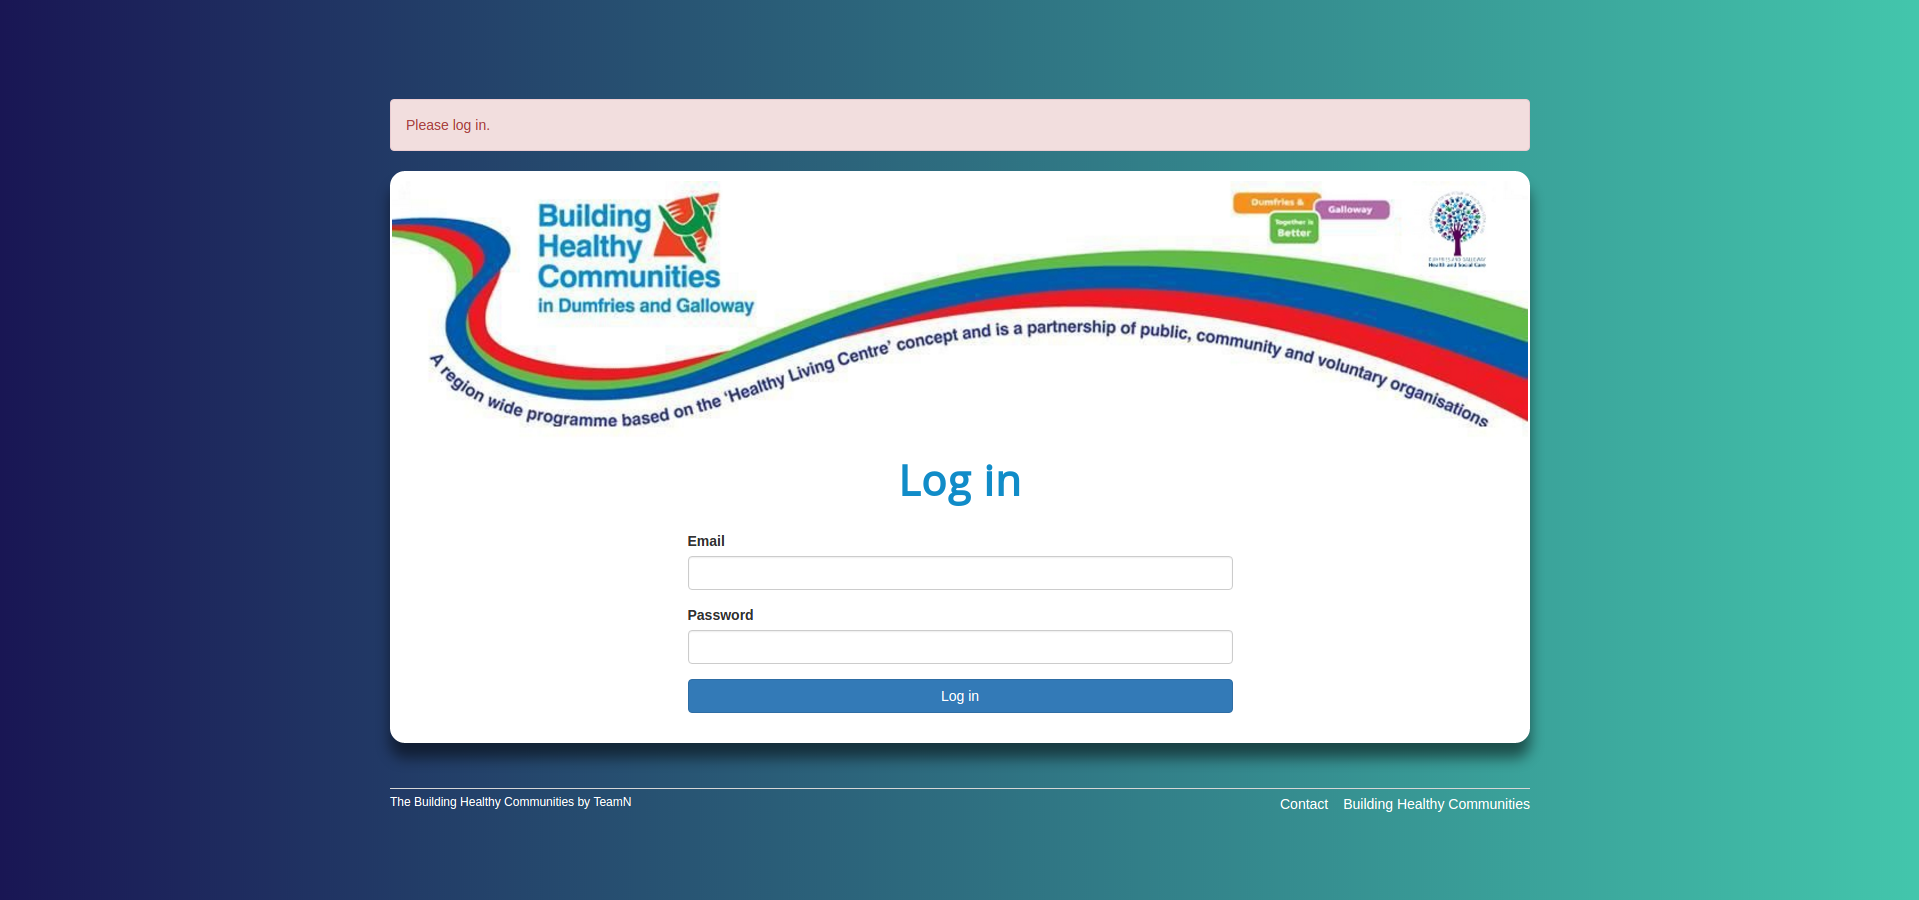
\includegraphics[width=\textwidth, height=\textheight, keepaspectratio]{loginscreen.png}}
 \caption{Login page}
 \label{fig:initialLogin}
\end{figure}

To login to the website, enter your email address and password. Until you do so, there is no way to access the website beyond this page. In the case that you have forgotten your email address and/or password, see \autoref{sec:contacts}: Contacts and Forgotten Passwords.

\pagebreak

\section{Home Page}
\label{sec:homepage}

\section{Profile}
\label{sec:profile}

\section{Data Tables}
\label{sec:datatables}

\section{Areas}
\label{sec:areas}

\section{Initiatives}
\label{sec:initiatives}

\section{Users}
\label{sec:users}

\section{Medical Conditions}
\label{sec:medical}

\section{Questions}
\label{sec:questions}

\section{Funders}
\label{sec:funders}

\section{Meetings}
\label{sec:meetings}

\section{Archives}
\label{sec:archives}

\section{Contacts and Forgotten Passwords}
\label{sec:contacts}

If you want to find contact details for a given area, there is an easy way to do so. On the login page (you will have to log out if you are currently logged in), in the bottom right is the word 'Contact'. Clicking on this will bring up the contacts page, from which the addresses of the various area partnerships can be found, as seen in \autoref{fig:contactPage}. This page also includes the names and roles of people working there, and a telephone number. If you have forgotten your email address and/or password, then you should contact another administrator directly, as the situation could pose a security risk. Other administrators can reset your account details, but should only do so with your explicit authorisation.

\begin{figure}[h]
 \centerline{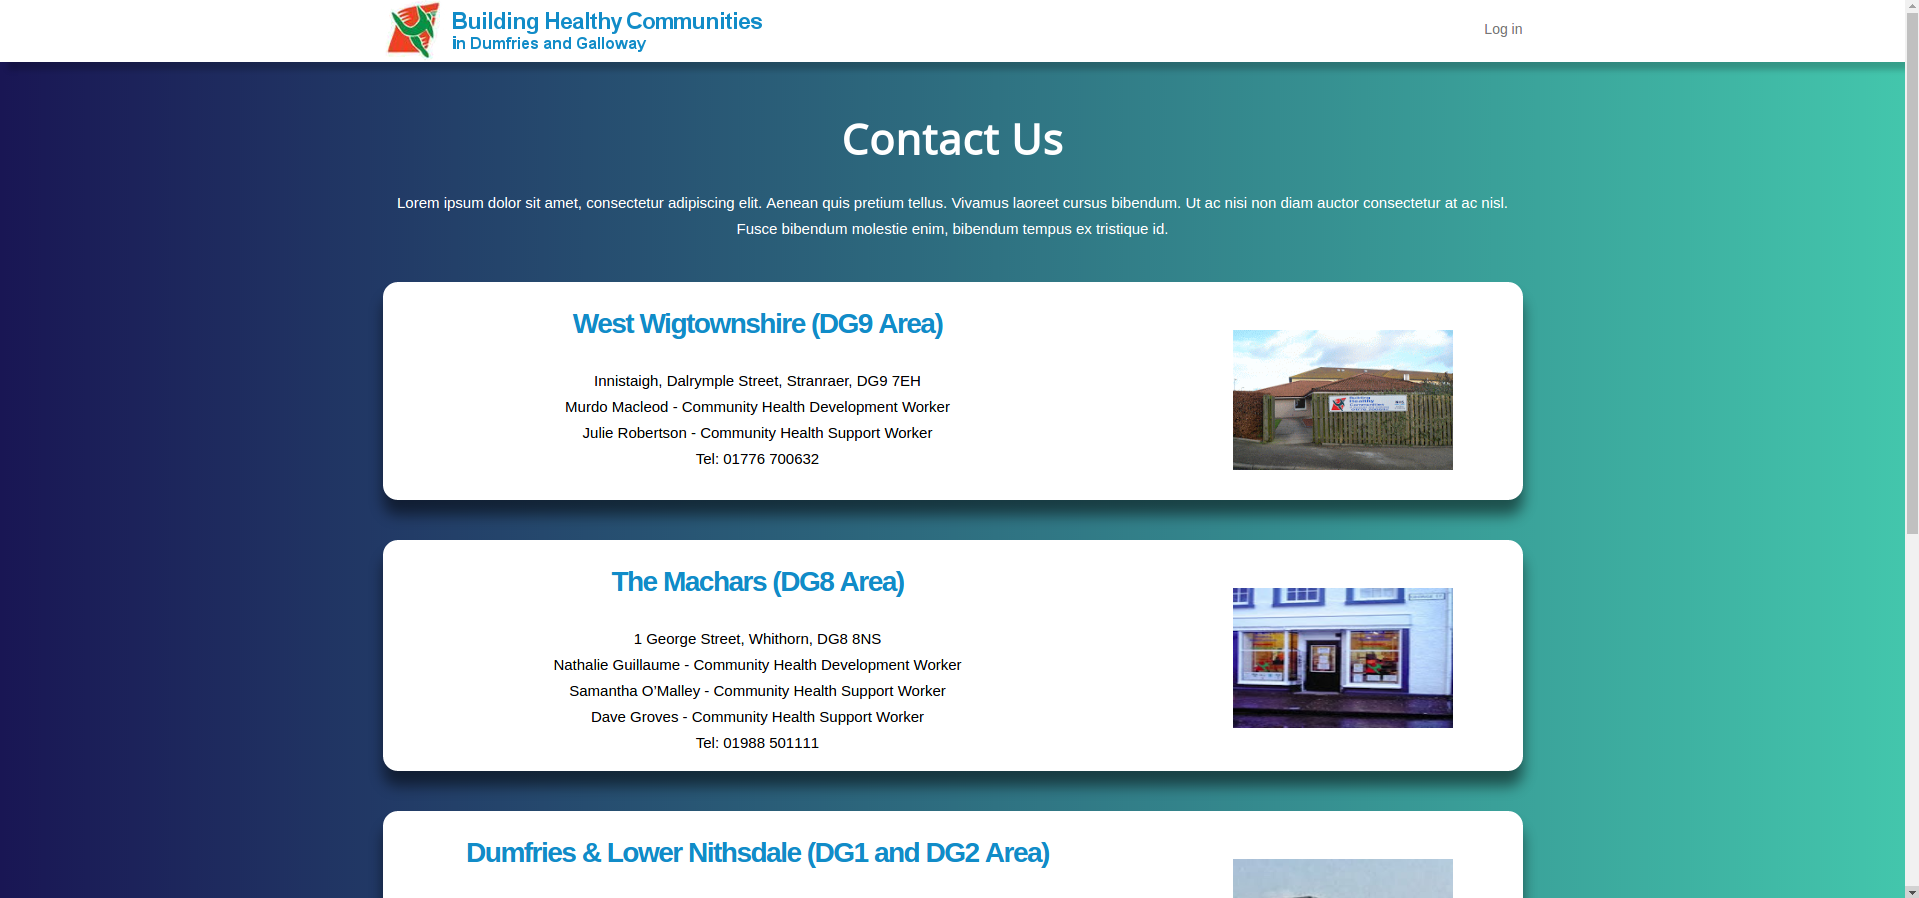
\includegraphics[width=\textwidth, height=\textheight, keepaspectratio]{contactpage.png}}
 \caption{Contact page}
 \label{fig:contactPage}
\end{figure}

\end{document}
